% Contenido de la presentación del TP5 (radar). Lo usan presentacion.tex y guion.tex.
% Cada diapositiva indica quién expone (\orador) y lo que dice (\note).
% Grupo Este procesó la señal 1 y Grupo Oeste la señal 2; la teoría se reparte entre los dos.

% =====================================================
% ---------- Portada ----------
% =====================================================
\begin{frame}[plain]
  \begin{tikzpicture}[remember picture, overlay]
    \node[anchor=east, xshift=1.2cm, yshift=-0.5cm, opacity=0.65] at (current page.east) {
      
\includegraphics[height=0.9\paperheight]{decoracion_a.png}
    };
    \fill[unc verde] (current page.north west) rectangle ([yshift=-1.6cm]current page.north east);
    \node[
      fill=unc verde, text=white, rounded corners=3pt,
      blur shadow={shadow blur steps=5, shadow xshift=0pt, shadow yshift=-3pt, shadow opacity=40},
      inner sep=12pt, minimum width=0.88\paperwidth, align=center, font=\Large\bfseries
    ] at ([yshift=-2.6cm]current page.north) {
      Sistemas de Radiocomunicación \\ Actividad 5: Radar
    };
    \node[anchor=center, text width=0.85\paperwidth, align=center] at ([yshift=-1.4cm]current page.center) {
      {\large\bfseries Teoría del radar y procesamiento de las señales 1 y 2}\\[0.25cm]
      {\normalsize Arteaga Barrera, Cristian Eduardo\\Baccino, Luca\\ Mendes Rosa, Agustín\\ Monja, Ernesto Joaquín}\\[0.25cm]
      {\small Facultad de Ciencias Exactas, Físicas y Naturales -- Universidad Nacional de Córdoba}\\[0.15cm]
      {\small Córdoba, 2026}
    };
    \node[anchor=south] at ([yshift=0.1cm]current page.south) {
      
\includegraphics[height=1.2cm]{unc_fcefyn_logo.png}
    };
  \end{tikzpicture}
  \orador{Grupo Este}{Cristian Arteaga Barrera}
  \note{\textbf{Cristian Arteaga Barrera (apertura):} Buenas. Somos Cristian Arteaga Barrera, Luca Baccino, Agustín Mendes Rosa y Joaquín Monja, y vamos a presentar la Actividad 5 de radar. Primero repasamos la teoría que pide la consigna y después mostramos el procesamiento de dos señales simuladas: la señal 1, que resolvimos Luca y yo, y la señal 2, que resolvieron Agustín y Joaquín.}
\end{frame}

% =====================================================
\section[Organización]{Organización}
\orador{Grupo Este}{Cristian Arteaga Barrera}
\begin{frame}{Organización de la exposición}
  \begin{columns}[T]
    \begin{column}{0.5\textwidth}
      \begin{block}{Señal 1}
        \small
        \textbf{Arteaga Barrera}
        \begin{itemize}
          \item El radar: definición, usos y diagrama en bloques
          \item Ecuación del radar, ruido y detección
        \end{itemize}
        \textbf{Baccino}
        \begin{itemize}
          \item Método: compresión, canceladores, CFAR y Doppler
          \item Resultados de la señal 1
        \end{itemize}
      \end{block}
    \end{column}
    \begin{column}{0.5\textwidth}
      \setbeamercolor{block title}{bg=grupo oeste,fg=white}
      \setbeamercolor{block body}{bg=grupo oeste!8}
      \begin{block}{Señal 2}
        \small
        \textbf{Mendes Rosa}
        \begin{itemize}
          \item Sección radar (RCS) y clutter
          \item Filtro apareado y señal chirp
        \end{itemize}
        \textbf{Monja}
        \begin{itemize}
          \item Resultados de la señal 2
          \item Comparación de las señales y conclusiones
        \end{itemize}
      \end{block}
    \end{column}
  \end{columns}
  \note{\textbf{Cristian Arteaga Barrera:} Nos organizamos así: yo presento qué es un radar y su ecuación; Agustín sigue con la sección radar, el clutter, el filtro apareado y el chirp. Después Luca explica el método de procesamiento, que es el mismo para las dos señales, y muestra los resultados de la señal 1. Cierra Joaquín con la señal 2, la comparación entre ambas y las conclusiones.}
\end{frame}

% =====================================================
\section[El radar]{El radar}
\orador{Grupo Este}{Cristian Arteaga Barrera}
\begin{frame}{¿Qué es un radar?}
  \textbf{RADAR}: \textit{RAdio Detection And Ranging}. Irradia ondas electromagnéticas y analiza los ecos de los blancos.
  \vspace{0.2cm}
  \begin{columns}[T]
    \begin{column}{0.5\textwidth}
      \begin{block}{Qué mide}
        \small
        \begin{itemize}
          \item \textbf{Distancia:} $R = \dfrac{c\,\Delta t}{2}$
          \item \textbf{Dirección:} apuntamiento de la antena
          \item \textbf{Velocidad radial:} $f_D = \dfrac{2 v_r}{\lambda}$
        \end{itemize}
        Funciona de día y de noche, con nubes, niebla o lluvia.
      \end{block}
    \end{column}
    \begin{column}{0.5\textwidth}
      \begin{block}{Usos}
        \small
        \begin{itemize}
          \item Control de tránsito aéreo
          \item Meteorología (lluvia, vientos)
          \item Navegación marítima y aérea
          \item Defensa: vigilancia y guiado
          \item SAR satelital (SAOCOM, banda L)
          \item Automotriz, cinemómetros
        \end{itemize}
      \end{block}
    \end{column}
  \end{columns}
  \note{\textbf{Cristian Arteaga Barrera:} Radar viene de \textit{Radio Detection And Ranging}. El radar emite una onda y escucha el eco que devuelven los objetos. La distancia sale del tiempo de ida y vuelta, dividido por dos porque la onda va y vuelve. La dirección la da hacia dónde apunta la antena, y la velocidad radial, el corrimiento Doppler. Como lleva su propia iluminación, funciona de noche y con mal tiempo. Se usa en control de tránsito aéreo, meteorología, navegación, defensa, en satélites de apertura sintética como los SAOCOM argentinos, y hasta en autos.}
\end{frame}

\begin{frame}{Parámetros típicos según la aplicación}
  \centering
  \small
  \renewcommand{\arraystretch}{1.15}
  \begin{tabular}{lllll}
    \toprule
    \textbf{Aplicación} & \textbf{Banda} & \textbf{Potencia pico} & \textbf{PRF} & \textbf{Alcance} \\
    \midrule
    Vigilancia aérea de ruta & L (1,2--1,4 GHz) & 1 a 5 MW & 300--400 Hz & 200--400 km \\
    Aproximación (ASR) & S (2,7--2,9 GHz) & $\approx$ 1 MW & $\approx$ 1 kHz & $\approx$ 100 km \\
    Meteorológico & S (2,7--3,0 GHz) & 750 kW & 318--1304 Hz & 460 km \\
    Navegación marítima & X (9,4 GHz) & 10 a 25 kW & 1--3 kHz & 50--100 km \\
    Automotriz (FMCW) & W (76--81 GHz) & $\approx$ 10 mW & continuo & 250 m \\
    \midrule
    \textbf{Este trabajo} & \textbf{L (1,3 GHz)} & -- & \textbf{1500 Hz} & \textbf{30 km} \\
    \bottomrule
  \end{tabular}
  \vspace{0.3cm}

  \raggedright\small
  Bandas bajas: menos atenuación y más alcance. Bandas altas: más resolución con antenas chicas, pero más atenuación por lluvia.
  \note{\textbf{Cristian Arteaga Barrera:} Los parámetros dependen de la aplicación. Los radares de largo alcance, como los de vigilancia de ruta, trabajan en banda L con potencias de megawatts y PRF bajas, porque necesitan mucho tiempo entre pulsos para escuchar ecos lejanos. Las bandas más altas dan mejor resolución con antenas chicas, pero sufren más atenuación por lluvia. El radar simulado del práctico está en banda L, a 1,3 GHz, con una PRF de 1500 Hz y una ventana de 30 km.}
\end{frame}

\begin{frame}{Diagrama en bloques de un radar pulsado}
  \centering
  \resizebox{\textwidth}{!}{%
  \begin{tikzpicture}[font=\footnotesize, node distance=0.6cm and 0.9cm,
      bloque/.style={draw, thick, rounded corners=2pt, fill=blue!8, minimum height=1.0cm, text width=2.3cm, align=center},
      flecha/.style={-{Stealth}, thick}]
      \node[bloque] (gen) {Generador de forma de onda};
      \node[bloque, right=of gen] (mod) {Modulador de pulsos};
      \node[bloque, right=of mod] (pa) {Amplificador de potencia};
      \node[bloque, right=of pa, fill=orange!15] (dup) {Duplexor};
      \node[right=1.2cm of dup] (ant) {\Large$\Psi$};
      \node[above=0.05cm of ant, font=\scriptsize] {Antena};
      \node[bloque, below=2.6cm of dup] (lna) {Amplificador de bajo ruido};
      \node[bloque, left=of lna] (mix) {Mezclador};
      \node[bloque, above=0.6cm of mix, fill=green!10] (ol) {Oscilador local};
      \node[bloque, left=of mix] (fi) {Amplificador de FI y filtro apareado};
      \node[bloque, left=of fi] (det) {Detector (demodulador I/Q)};
      \node[bloque, below=1.0cm of det, fill=purple!10] (proc) {Procesador de señal: MTI, Doppler, CFAR};
      \node[bloque, right=of proc, fill=purple!10] (datos) {Procesador de datos: detección y seguimiento};
      \node[bloque, right=of datos] (disp) {Presentación (display)};
      \node[bloque, below=0.7cm of gen, fill=yellow!20] (sinc) {Sincronizador (PRF)};
      \draw[flecha] (gen) -- (mod); \draw[flecha] (mod) -- (pa); \draw[flecha] (pa) -- (dup);
      \draw[{Stealth}-{Stealth}, thick] (dup) -- (ant);
      \draw[flecha] (dup) -- (lna); \draw[flecha] (lna) -- (mix); \draw[flecha] (ol) -- (mix);
      \draw[flecha] (mix) -- (fi); \draw[flecha] (fi) -- (det); \draw[flecha] (det) -- (proc);
      \draw[flecha] (proc) -- (datos); \draw[flecha] (datos) -- (disp);
      \draw[flecha, dashed] (sinc) -- (gen);
      \draw[flecha, dashed] (sinc.west) -- ++(-0.35,0) |- (proc.west);
  \end{tikzpicture}}
  \note{\textbf{Cristian Arteaga Barrera:} Este es el diagrama de un radar pulsado. El sincronizador marca la PRF de todo el sistema. El generador arma el pulso, por ejemplo un chirp, el modulador lo enciende y apaga, y el amplificador de potencia lo lleva a la potencia pico. El duplexor conecta la antena al transmisor o al receptor y protege al receptor mientras se transmite; por eso hay un rango mínimo en el que el radar está ciego. En recepción, el amplificador de bajo ruido fija la figura de ruido, el mezclador baja la señal y el filtro apareado maximiza la relación señal a ruido. El detector I/Q conserva la fase, que hace falta para el Doppler. Después el procesador de señal cancela el clutter, separa por velocidad y decide con un umbral CFAR, que es justamente lo que hicimos en el práctico.}
\end{frame}

\begin{frame}{Ecuación del radar y relación señal a ruido}
  \begin{block}{Potencia recibida}
    \[
      P_r = \frac{P_t G}{4\pi R^2} \cdot \frac{\sigma}{4\pi R^2} \cdot \frac{G\lambda^2}{4\pi} \cdot \frac{1}{L}
          = \frac{P_t\, G^2 \lambda^2 \sigma}{(4\pi)^3 R^4 L}
    \]
  \end{block}
  \begin{block}{Con el ruido del receptor $N = k T_s B_n$}
    \[
      SNR = \frac{P_t\, G^2 \lambda^2 \sigma}{(4\pi)^3 R^4\, k T_s B_n L}
      \qquad
      R_{max} = \left[\frac{P_t\, G^2 \lambda^2 \sigma}{(4\pi)^3\, k T_s B_n L\, SNR_{min}}\right]^{1/4}
    \]
  \end{block}
  \small
  \begin{itemize}
    \item El factor $R^{-4}$ viene de la doble dispersión: \textbf{duplicar el alcance exige 16 veces más potencia}.
  \end{itemize}
  \note{\textbf{Cristian Arteaga Barrera:} La ecuación del radar se arma por partes: la densidad de potencia que llega al blanco, lo que el blanco reirradia según su sección radar sigma, que vuelve a dispersarse en una esfera, y lo que capta el área efectiva de la antena. El resultado depende de la cuarta potencia de la distancia, así que para duplicar el alcance hace falta dieciséis veces más potencia. Si dividimos por el ruido del receptor, k por la temperatura de sistema por el ancho de banda, obtenemos la relación señal a ruido, y despejando, el alcance máximo para la SNR mínima que pide la detección.}
\end{frame}

\begin{frame}{Detección: falsa alarma, detección e integración}
  \begin{columns}[T]
    \begin{column}{0.5\textwidth}
      \begin{block}{Umbral y probabilidades}
        \small
        La envolvente del ruido es de Rayleigh:
        \[ P_{fa} = e^{-V_T^2/2\psi_0} \]
        \begin{itemize}
          \item $P_{fa}$: declarar un blanco donde solo hay ruido. Fija el umbral.
          \item $P_d$: que blanco + ruido (Rice) supere el umbral. Crece con la SNR.
          \item $P_d = 0{,}9$ y $P_{fa} = 10^{-6}$ requieren $\approx 13{,}2$ dB.
        \end{itemize}
      \end{block}
    \end{column}
    \begin{column}{0.5\textwidth}
      \begin{block}{Integración de $n$ pulsos}
        \small
        \begin{itemize}
          \item \textbf{Coherente:} suma amplitud y fase, $SNR_n = n \cdot SNR_1$.
          \item \textbf{No coherente:} suma envolventes, ganancia $\approx n^{0{,}7}$ a $n^{0{,}8}$.
        \end{itemize}
        \[ R_{max} \propto \left(n E_i(n)\right)^{1/4} \]
      \end{block}
    \end{column}
  \end{columns}
  \note{\textbf{Cristian Arteaga Barrera:} Como el ruido es aleatorio, detectar es un problema estadístico. Se compara la envolvente con un umbral. La probabilidad de falsa alarma es la de que el ruido solo pase el umbral, y es la que lo fija. La probabilidad de detección es la de que el blanco más ruido lo supere, y crece con la SNR: por ejemplo, para noventa por ciento de detección con una falsa alarma en un millón hacen falta unos 13 dB. Como el radar recibe varios ecos del mismo blanco, se pueden integrar: la integración coherente, que suma con la fase, multiplica la SNR por la cantidad de pulsos; la no coherente gana menos. Con esto le paso la palabra a Agustín.}
\end{frame}

% =====================================================
\section[RCS y clutter]{RCS y clutter}
\orador{Grupo Oeste}{Agustín Mendes Rosa}
\begin{frame}{Sección radar (RCS)}
  \begin{block}{Definición}
    Área ficticia que, reirradiando isotrópicamente la potencia que intercepta, daría el mismo eco que el blanco real:
    \[ \sigma = \lim_{R\to\infty} 4\pi R^2 \frac{|E_s|^2}{|E_i|^2} \quad [m^2] \]
  \end{block}
  \small
  \begin{itemize}
    \item No es el área física: depende de la frecuencia, la polarización, la forma, el material y el ángulo.
    \item Valores típicos: insecto $10^{-5}$ m$^2$, avión liviano 1 m$^2$, avión de pasajeros 100 m$^2$, buque $10^4$ m$^2$.
    \item Blancos complejos: suma de muchos dispersores, la RCS varía decenas de dB con el ángulo. Se mide (campo abierto, cámara anecoica, modelos a escala) o se calcula (óptica física, método de los momentos).
  \end{itemize}
  \note{\textbf{Agustín Mendes Rosa:} La sección radar es el área equivalente que, si reirradiara en todas direcciones lo que intercepta, produciría el mismo eco que el blanco. No es el tamaño físico: depende de la frecuencia, la forma, el material y el ángulo de observación. Va de una cien milésima de metro cuadrado para un insecto a diez mil para un barco. En un avión o un barco hay muchos dispersores cuyas contribuciones se suman con fases que cambian con el ángulo, así que su RCS se mide en polígonos o cámaras anecoicas, o se calcula con métodos electromagnéticos.}
\end{frame}

\begin{frame}{RCS de dos blancos simples}
  \begin{columns}[T]
    \begin{column}{0.5\textwidth}
      \centering
      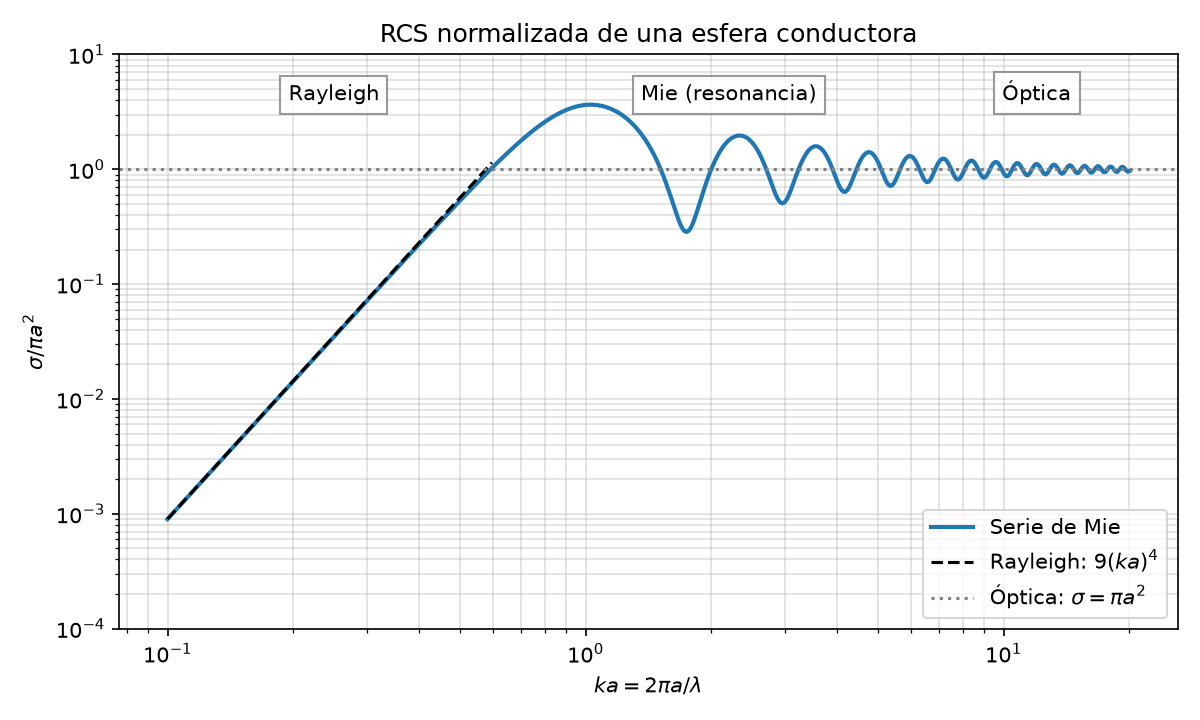
\includegraphics[width=\textwidth]{teoria/rcs_esfera.png}

      \raggedright\footnotesize
      \textbf{Esfera:} Rayleigh ($\sigma \propto f^4$), resonancia de Mie y región óptica ($\sigma \to \pi a^2$).
    \end{column}
    \begin{column}{0.5\textwidth}
      \centering
      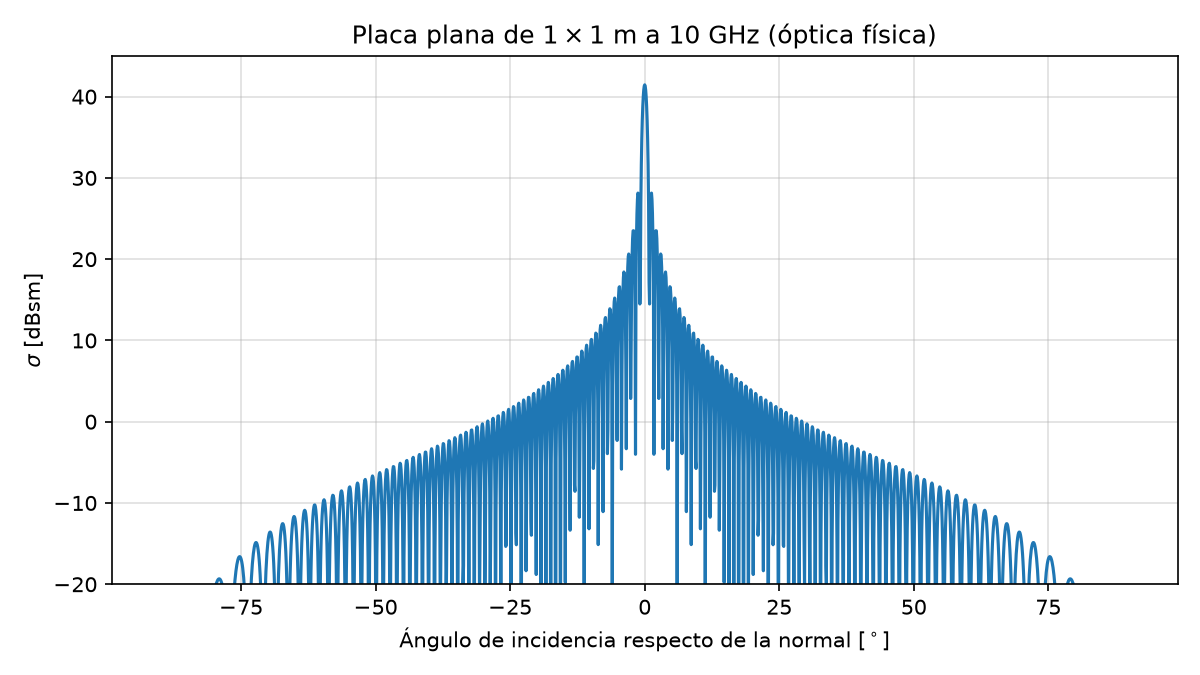
\includegraphics[width=\textwidth]{teoria/rcs_placa.png}

      \raggedright\footnotesize
      \textbf{Placa plana} $1 \times 1$ m a 10 GHz: $\sigma_{max} = 4\pi A^2/\lambda^2 = 41{,}4$ dBsm en la normal; a pocos grados cae más de 30 dB.
    \end{column}
  \end{columns}
  \note{\textbf{Agustín Mendes Rosa:} Calculamos la RCS de dos blancos simples. La esfera es la referencia, porque no depende del ángulo. Con la serie de Mie se ven tres regiones: cuando la esfera es chica frente a la longitud de onda, la RCS crece con la cuarta potencia de la frecuencia, y por eso la lluvia refleja más en bandas altas; en la zona de resonancia oscila; y cuando es grande tiende al área de su sección, pi a cuadrado. La placa plana, en cambio, se comporta como un espejo: de frente tiene una RCS enorme, más de 41 dBsm para un metro cuadrado a 10 GHz, pero apenas se inclina unos grados cae más de 30 dB. Es el principio de los aviones furtivos, que orientan sus superficies lejos del radar.}
\end{frame}

\begin{frame}{Clutter}
  Ecos no deseados de objetos que no son los blancos de interés. A diferencia del ruido, \textbf{es eco de la propia señal}: crece con la potencia y está correlacionado entre pulsos. Puede superar al blanco en 50 o 60 dB.
  \vspace{0.15cm}
  \small
  \begin{columns}[T]
    \begin{column}{0.5\textwidth}
      \begin{itemize}
        \item \textbf{Terrestre:} suelo, edificios, árboles. Doppler angosto en cero.
        \item \textbf{Mar:} depende del estado del mar; picos (\textit{sea spikes}).
        \item \textbf{Meteorológico:} lluvia y granizo, $\propto f^4$; se mueve con el viento.
      \end{itemize}
    \end{column}
    \begin{column}{0.5\textwidth}
      \begin{itemize}
        \item \textbf{Chaff:} dipolos de $\lambda/2$ como contramedida.
        \item \textbf{Biológico:} aves e insectos (``ángeles'').
        \item \textbf{Discreto:} torres, aerogeneradores, vehículos.
      \end{itemize}
    \end{column}
  \end{columns}
  \vspace{0.2cm}
  \begin{block}{En las señales del práctico}
    \small Clutter cercano entre 1,5 y 2,5 km en todas las señales: lo elimina el cancelador MTI.
  \end{block}
  \note{\textbf{Agustín Mendes Rosa:} El clutter son los ecos que no nos interesan: el suelo, el mar, la lluvia, las aves o el chaff, que son nubes de dipolos que se tiran como contramedida. La diferencia con el ruido es que es un eco de nuestra propia señal: si subimos la potencia, sube igual, y se parece de un pulso al siguiente. Puede ser 50 o 60 dB más fuerte que el blanco. La forma de separarlo es por velocidad: el clutter de tierra tiene Doppler casi nulo. En las señales del práctico hay clutter cercano entre 1,5 y 2,5 km, y lo elimina el cancelador MTI, como va a mostrar Luca.}
\end{frame}

\begin{frame}{Filtro apareado}
  \begin{columns}[T]
    \begin{column}{0.52\textwidth}
      \begin{block}{Definición y derivación (AWGN)}
        \small
        Filtro lineal que maximiza la SNR en $t_0$. Por la desigualdad de Schwarz:
        \[ SNR(t_0) \leq \frac{2E}{N_0} \]
        con igualdad si
        \[ H(f) = K S^*(f) e^{-j2\pi f t_0} \;\Leftrightarrow\; h(t) = K s^*(t_0 - t) \]
      \end{block}
    \end{column}
    \begin{column}{0.48\textwidth}
      \begin{block}{Propiedades}
        \small
        \begin{itemize}
          \item La SNR máxima depende solo de la energía, no de la forma.
          \item La salida es la autocorrelación de la señal.
          \item El pico mide $\approx 1/B$: base de la compresión.
          \item Ruido no blanco: $H = K S^*/N_i$ (blanqueo + apareado).
        \end{itemize}
      \end{block}
    \end{column}
  \end{columns}
  \note{\textbf{Agustín Mendes Rosa:} El filtro apareado es el filtro lineal que maximiza la relación señal a ruido en un instante. Con ruido blanco, la desigualdad de Schwarz da que la SNR no puede superar dos veces la energía sobre N cero, y ese máximo se alcanza cuando el filtro es la señal invertida en el tiempo y conjugada. Lo importante es que la SNR depende solo de la energía, no de la forma, y que el pico de salida es tan angosto como la inversa del ancho de banda. Si el ruido no es blanco, por ejemplo con clutter o interferencias, el filtro óptimo primero blanquea el ruido y después aparea.}
\end{frame}

\begin{frame}{Señal chirp y compresión de pulsos}
  \centering
  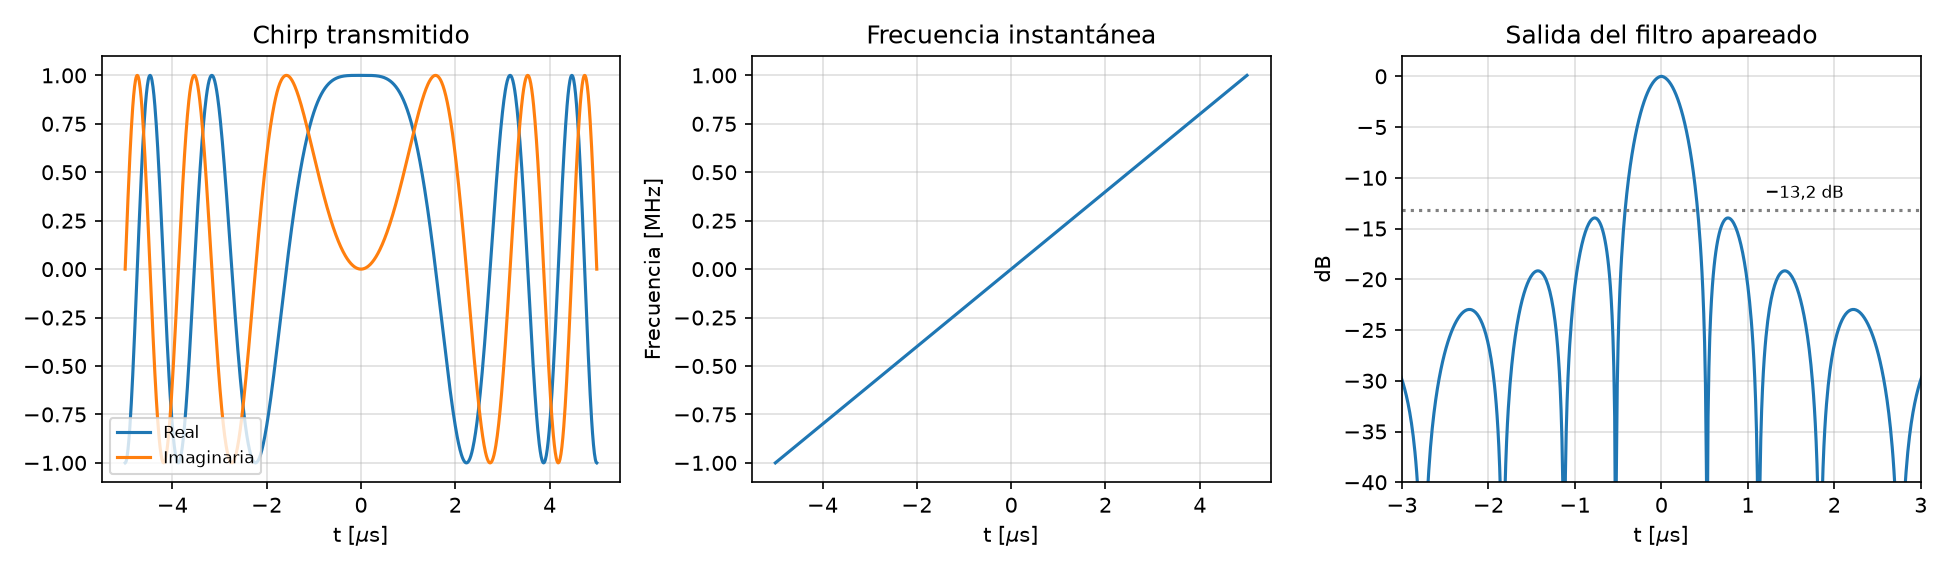
\includegraphics[width=\textwidth]{teoria/chirp_compresion.png}
  \vspace{-0.1cm}
  \raggedright\small
  \begin{columns}[T]
    \begin{column}{0.5\textwidth}
      \[ s(t) = \mathrm{rect}\!\left(\frac{t}{T}\right) e^{j\pi \frac{B}{T} t^2}, \quad f_i(t) = \frac{B}{T}\,t \]
      Energía según $T$, resolución según $B$.
    \end{column}
    \begin{column}{0.5\textwidth}
      \begin{itemize}
        \item Sin comprimir: $cT/2 = 1500$ m
        \item Comprimido: $\Delta R = c/2B = \mathbf{75}$ \textbf{m}
        \item $BT = 20$: 13 dB de ganancia
      \end{itemize}
    \end{column}
  \end{columns}
  \note{\textbf{Agustín Mendes Rosa:} En un pulso simple hay un compromiso: más largo da más energía y más alcance, pero peor resolución. El chirp lo resuelve modulando la frecuencia linealmente durante el pulso: la energía la da la duración y la resolución, el ancho de banda. Al pasar por el filtro apareado todas las frecuencias se alinean y el pulso de 10 microsegundos se comprime en un pico de ancho uno sobre B. En el práctico, con 2 MHz, la resolución pasa de 1500 metros a 75, veinte veces mejor, con 13 dB de ganancia. Gracias a eso se separan blancos a 300 metros. Ahora sigue Luca con el procesamiento.}
\end{frame}

% =====================================================
\section[Método]{Método}
\orador{Grupo Este}{Luca Baccino}
\begin{frame}{Datos y parámetros del radar simulado}
  \small
  Cada señal: \textbf{100 pulsos $\times$ 2000 muestras I/Q} (de 15 m a 30 km, paso de 15 m), con 2 a 10 blancos desconocidos.\par
  \vspace{0.2cm}
  \centering
  \renewcommand{\arraystretch}{1.1}
  \begin{tabular}{lr|lr}
    \toprule
    \textbf{Parámetro} & \textbf{Valor} & \textbf{Derivado} & \textbf{Valor} \\
    \midrule
    $f_c$ & 1,3 GHz & $\lambda$ & 23,1 cm \\
    $f_s$ & 10 MHz & Paso en rango & 15 m \\
    $T_p$ & 10 $\mu$s & Resolución $c/2B$ & 75 m \\
    $B$ & 2 MHz & $BT$ & 20 (13 dB) \\
    PRF & 1500 Hz & Rango mínimo & 1,5 km \\
    $N_p$ & 100 & Rango no ambiguo & 97,75 km \\
    Ventana & 30 km & Velocidad no ambigua & $\pm 86{,}5$ m/s \\
    \bottomrule
  \end{tabular}
  \note{\textbf{Luca Baccino:} Cada señal tiene 100 pulsos de 2000 muestras complejas. La ordenamos en una matriz: las filas son el tiempo lento, de un pulso al siguiente, y las columnas el tiempo rápido, que es el rango, de 15 metros a 30 kilómetros. De los parámetros salen las magnitudes que vamos a usar: la resolución de 75 metros, el rango mínimo de 1,5 km, porque el receptor está ciego durante el pulso y la recuperación, y la velocidad no ambigua de más o menos 86,5 metros por segundo, que la fija la PRF. El procesamiento es el mismo para las dos señales y está en el script tp5\_radar.py, basado en el código de la cátedra.}
\end{frame}

\begin{frame}{Cadena de procesamiento}
  \centering
  \resizebox{\textwidth}{!}{%
  \begin{tikzpicture}[font=\footnotesize,
        b/.style={draw, thick, rounded corners=2pt, fill=blue!8, minimum height=1.0cm, text width=2.5cm, align=center},
        f/.style={-{Stealth}, thick}]
        \node[b] (raw) at (0, 0) {Datos crudos\\$100 \times 2000$};
        \node[b] (mf) at (3.4, 0) {Filtro apareado\\(compresión)};
        \node[b, fill=orange!12] (mti) at (7.0, 1.8) {MTI SC\\$1 - z^{-1}$};
        \node[b, fill=orange!12] (sti) at (7.0, 0) {STI SC\\$1 + z^{-1}$};
        \node[b, fill=orange!12] (dc) at (7.0, -1.8) {MTI DC\\$1 - 2z^{-1} + z^{-2}$};
        \node[b, fill=green!10] (dop) at (10.6, 3.6) {Filtrado Doppler\\(DFT en tiempo lento)};
        \node[b, fill=green!10] (c1) at (10.6, 1.8) {CFAR y\\cruces por cero};
        \node[b, fill=green!10] (c2) at (10.6, 0) {CFAR y\\cruces por cero};
        \node[b, fill=green!10] (c3) at (10.6, -1.8) {CFAR y\\cruces por cero};
        \node[b, fill=purple!10] (vel) at (14.2, 3.6) {Velocidad de\\blancos móviles};
        \node[b, fill=purple!10] (r1) at (14.2, 1.8) {Rango de\\blancos móviles};
        \node[b, fill=purple!10] (r2) at (14.2, 0) {Rango de\\blancos fijos};
        \node[b, fill=purple!10] (r3) at (14.2, -1.8) {Rango de\\blancos móviles};
        \draw[f] (raw) -- (mf);
        \draw[f] (mf) -- (sti);
        \draw[f] (mf.east) -- ++(0.45,0) |- (mti.west);
        \draw[f] (mf.east) -- ++(0.45,0) |- (dc.west);
        \draw[f] (mti.north) |- (dop.west);
        \draw[f] (mti) -- (c1); \draw[f] (sti) -- (c2); \draw[f] (dc) -- (c3);
        \draw[f] (dop) -- (vel); \draw[f] (c1) -- (r1); \draw[f] (c2) -- (r2); \draw[f] (c3) -- (r3);
    \end{tikzpicture}}
  \vspace{0.3cm}

  \raggedright\small
  Validado con la señal de ejemplo: blancos en 10,02, 15,02 y 20,01 km (consigna: 9,95, 14,97 y 19,93 km) y un fijo en 18,02 km.
  \note{\textbf{Luca Baccino:} Esta es la cadena completa. Primero se comprime cada pulso con el filtro apareado. Después se aplican los tres canceladores entre pulsos: MTI simple, STI simple y MTI doble. A la salida de cada uno se aplica el CFAR y se detecta con cruces por cero, lo que da el rango de los blancos. En paralelo, la salida del MTI pasa por el filtrado Doppler, que da la velocidad de los móviles. Antes de procesar nuestras señales lo probamos con la señal de ejemplo de la consigna y encontramos los mismos tres blancos, con diferencias de menos de 80 metros.}
\end{frame}

\begin{frame}{1. Compresión con filtro apareado}
  \begin{columns}[c]
    \begin{column}{0.58\textwidth}
      \centering
      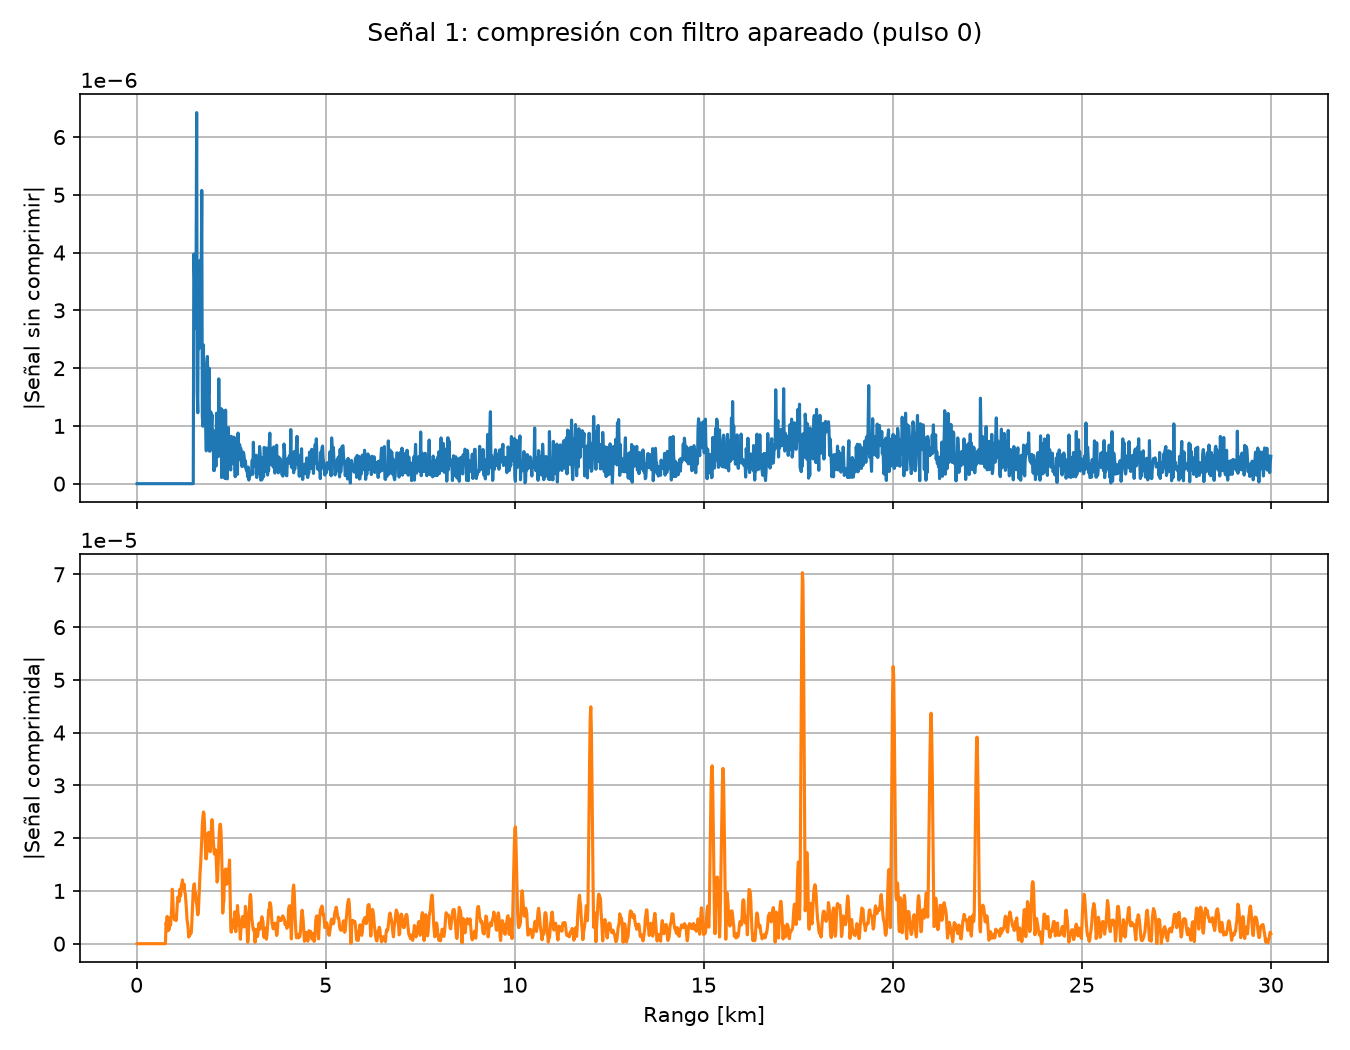
\includegraphics[height=0.78\textheight]{senal_1/02_compresion.png}
    \end{column}
    \begin{column}{0.42\textwidth}
      \small
      \[ h(t) = s^*(-t) \]
      \[ y_p = \mathrm{IFFT}\{X_p(f)\, S^*(f)\} \]
      \begin{itemize}
        \item Convolución por FFT (\texttt{fastconv}).
        \item Se conservan las 2000 muestras centrales para alinear el pico con el rango.
        \item Sin comprimir, los ecos quedan bajo el ruido; comprimidos, emergen 8 picos.
      \end{itemize}
    \end{column}
  \end{columns}
  \note{\textbf{Luca Baccino:} El primer paso es la compresión. Generamos el mismo chirp que transmite el radar, lo invertimos y conjugamos, y convolucionamos cada pulso con él usando la FFT. La convolución sale más larga, así que recortamos las muestras centrales para que cada pico quede en su distancia; lo verificamos con un eco sintético a 10 km. Arriba se ve la señal cruda: los ecos están debajo del ruido. Abajo, después de comprimir, aparecen claramente ocho picos en la señal 1.}
\end{frame}

\begin{frame}{2. Canceladores en tiempo lento}
  \begin{columns}[c]
    \begin{column}{0.44\textwidth}
      \small
      \begin{itemize}
        \item \textbf{MTI simple:} $x_p - x_{p-1}$ \\ $|H| = 2|\sin(\pi f_D/PRF)|$
        \item \textbf{STI simple:} $x_p + x_{p-1}$ \\ $|H| = 2|\cos(\pi f_D/PRF)|$
        \item \textbf{MTI doble:} $x_p - 2x_{p-1} + x_{p-2}$ \\ $|H| = 4\sin^2(\pi f_D/PRF)$
      \end{itemize}
      MTI: pasaaltos (elimina lo fijo). STI: pasabajos (refuerza lo fijo). \\
      Velocidades ciegas: $v_b = k\,\lambda\,PRF/2 = k \cdot 173$ m/s.
    \end{column}
    \begin{column}{0.56\textwidth}
      \centering
      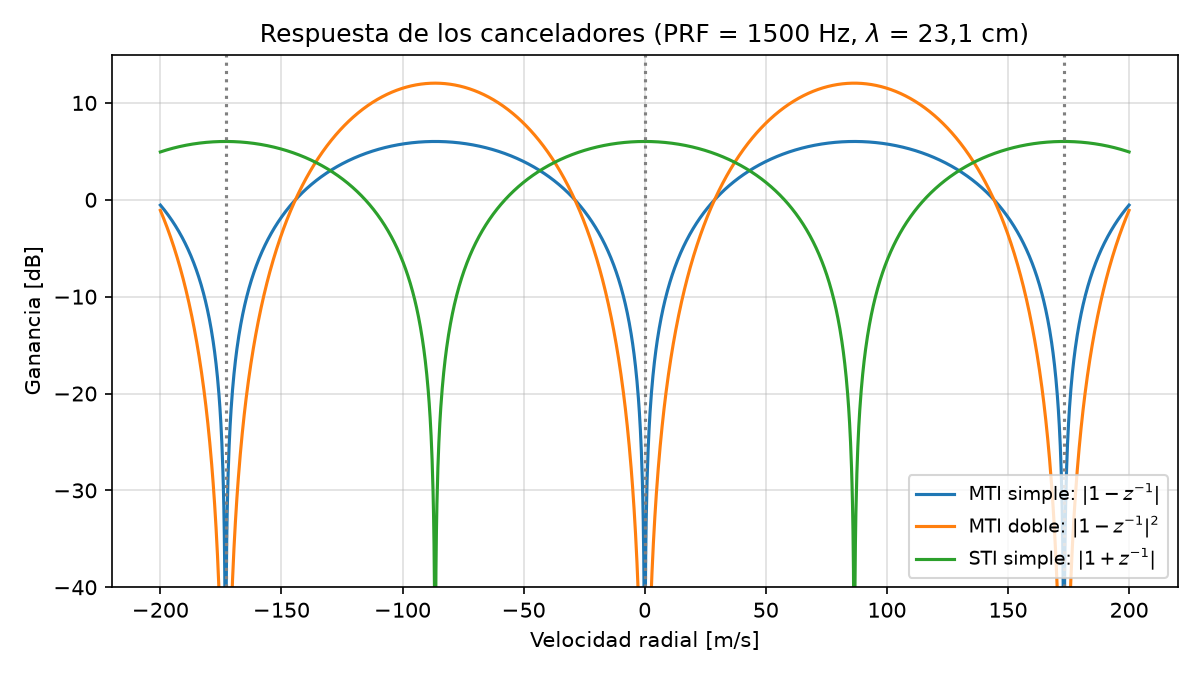
\includegraphics[width=\textwidth]{teoria/respuesta_canceladores.png}
    \end{column}
  \end{columns}
  \note{\textbf{Luca Baccino:} Los canceladores comparan cada pulso con el anterior en la misma celda de rango. Si el blanco está quieto, el eco es igual en todos los pulsos y el MTI, que resta, lo anula; si se mueve, la fase cambia y queda un residuo. El STI suma, así que hace lo contrario: refuerza lo quieto. El doble cancelador es el MTI aplicado dos veces y tiene un nulo más ancho en velocidad cero. En el gráfico se ve que la respuesta se repite cada PRF: un blanco a 173 metros por segundo es invisible para el MTI, son las velocidades ciegas. Y el STI tiene su nulo en la mitad, cerca de 86 metros por segundo.}
\end{frame}

\begin{frame}{3. Umbral CA-CFAR y detección}
  \begin{columns}[c]
    \begin{column}{0.48\textwidth}
      \centering
      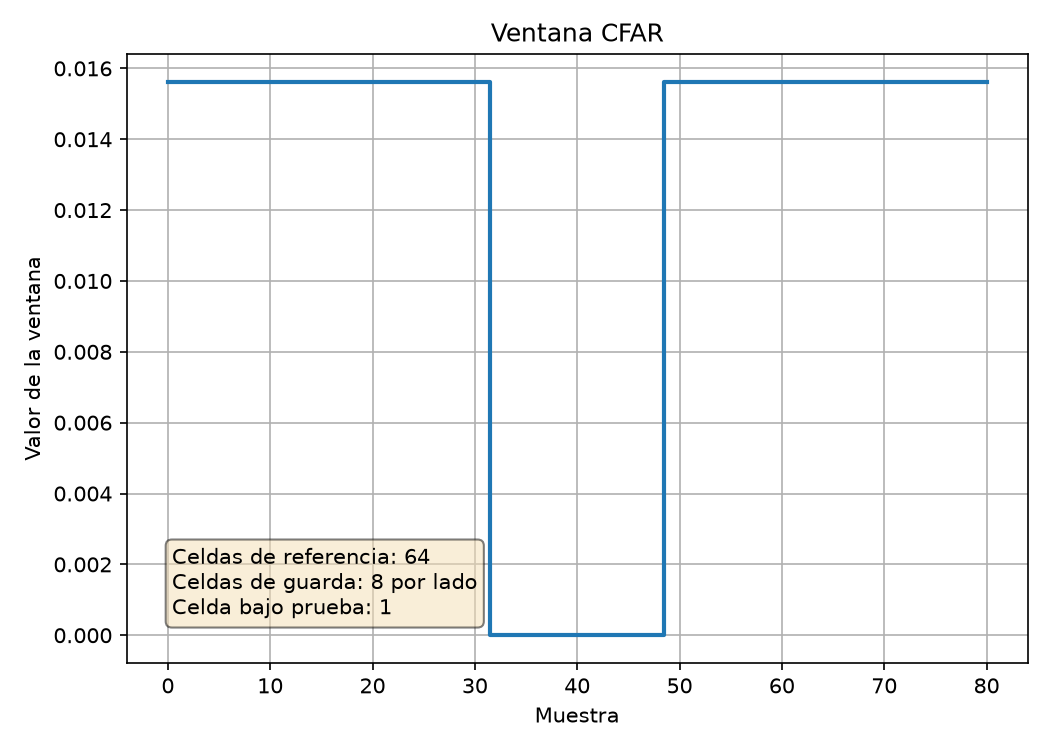
\includegraphics[width=\textwidth]{senal_1/03_ventana_cfar.png}
    \end{column}
    \begin{column}{0.52\textwidth}
      \small
      \begin{itemize}
        \item Ruido local: promedio de $N_R = 64$ celdas de referencia, con $N_G = 8$ de guarda por lado.
        \item $P_{fa} = 10^{-6}$: $\alpha = N_R\left(P_{fa}^{-1/N_R} - 1\right) = 15{,}4$
        \item Ganancia en amplitud: $\sqrt{\alpha} = \mathbf{3{,}93}$.
        \item Cruces por cero: $\Delta\,\mathrm{sign}(|y| - V_T)$ vale $+2$ al inicio y $-2$ al fin de cada detección.
        \item 200 celdas (ejemplo de la cátedra) enmascaraban blancos cercanos.
      \end{itemize}
    \end{column}
  \end{columns}
  \note{\textbf{Luca Baccino:} Para decidir si hay un blanco usamos un CFAR de promedio de celdas. Para cada celda estimamos el ruido como el promedio de 64 vecinas, 32 de cada lado, dejando 8 de guarda para que el propio blanco no infle la estimación. El umbral es ese ruido por alfa; con una falsa alarma en un millón, alfa da 15,4, que en amplitud es una ganancia de 3,93. La detección se hace con cruces por cero: el signo de la salida menos el umbral, derivado, vale más dos donde empieza una detección y menos dos donde termina. Probamos con las 200 celdas del ejemplo de la cátedra, pero un blanco fuerte tapaba a los vecinos, así que achicamos la ventana.}
\end{frame}

\begin{frame}{4. Filtrado Doppler y clasificación}
  \begin{columns}[T]
    \begin{column}{0.5\textwidth}
      \begin{block}{DFT en tiempo lento}
        \small
        \[ \mathbf{Y} = \mathbf{MTI}_{SC}^{\,T}\,\mathbf{F_D}, \quad F_D[r,c] = e^{-j2\pi rc/m} \]
        \begin{itemize}
          \item $m = 99$ pulsos: integración coherente ($\approx 20$ dB).
          \item $v_r = f_D\,\lambda/2$, resolución 1,75 m/s.
          \item CFAR por velocidad sobre el mapa, con ventana de Hamming (lóbulos de $-13$ a $-43$ dB).
        \end{itemize}
      \end{block}
    \end{column}
    \begin{column}{0.5\textwidth}
      \begin{block}{Clasificación}
        \small
        \begin{itemize}
          \item \textbf{Móvil:} detección Doppler confirmada por un cancelador o con SNR $\geq 20$ dB.
          \item \textbf{Fijo:} el STI supera al MTI en más de 10 dB.
          \item \textbf{Residuo:} 20 dB debajo de otro blanco en la misma celda.
          \item \textbf{Falsa alarma:} débil y sin confirmar.
        \end{itemize}
      \end{block}
    \end{column}
  \end{columns}
  \note{\textbf{Luca Baccino:} Para obtener las velocidades tomamos la salida del MTI y multiplicamos por la matriz de la DFT, como pide la consigna. Así cada celda de rango tiene su espectro Doppler, y cada frecuencia se convierte en velocidad con f D por lambda sobre dos. Además, sumar 99 pulsos con su fase da casi 20 dB de ganancia. Sobre ese mapa aplicamos el mismo CFAR, con una ventana de Hamming para que los blancos fuertes no generen detecciones falsas en otras velocidades. Finalmente clasificamos: móviles los confirmados, fijos los que el STI ve mucho más fuerte que el MTI, y descartamos residuos y falsas alarmas.}
\end{frame}

% =====================================================
\section[Señal 1]{Señal 1}
\orador{Grupo Este}{Luca Baccino}
\begin{frame}{Señal 1: CFAR del MTI simple cancelador}
  \begin{columns}[c]
    \begin{column}{0.5\textwidth}
      \centering
      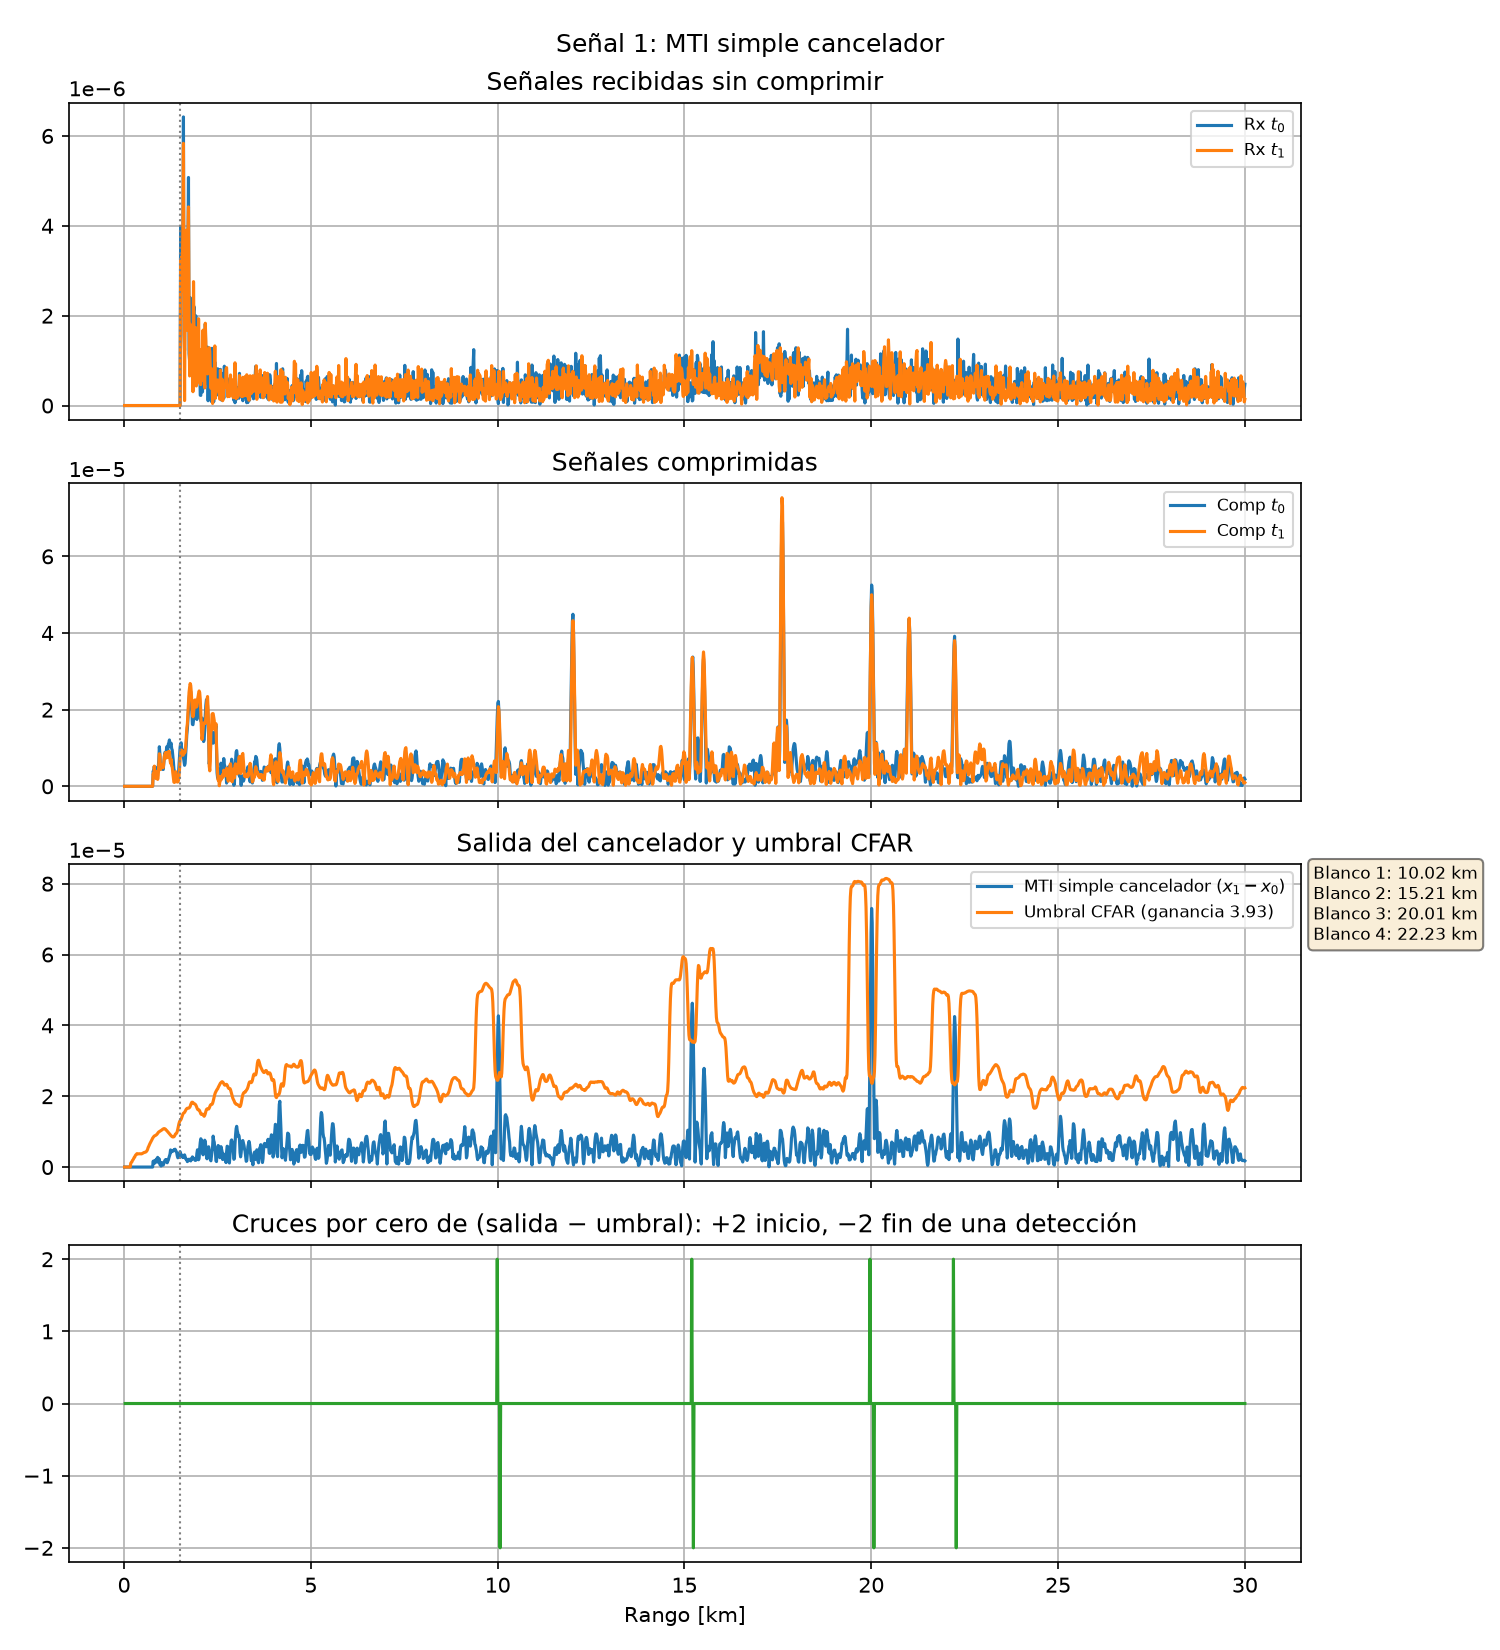
\includegraphics[height=0.86\textheight]{senal_1/04_cfar_mti_sc.png}
    \end{column}
    \begin{column}{0.5\textwidth}
      \small
      \textbf{Rangos detectados [km]:}
      \begin{itemize}
        \item MTI simple: 10,02 -- 15,21 -- 20,01 -- 22,23
        \item MTI doble: igual
        \item STI simple: 12,02 -- 17,61 -- 20,01 -- 21,02 -- 22,23
      \end{itemize}
      \begin{itemize}
        \item El MTI cancela el clutter y los ecos fijos de 12,02, 17,61 y 21,02 km.
        \item El STI no ve el de 10,02 km: $f_D = -742$ Hz, cerca de $-PRF/2$ (nulo de $\approx 30$ dB).
        \item 15,51 km queda enmascarado por el de 15,21 km (a 300 m).
      \end{itemize}
    \end{column}
  \end{columns}
  \note{\textbf{Luca Baccino:} Acá está la salida del MTI simple de la señal 1, con el umbral CFAR en naranja y los cruces por cero abajo. Detecta cuatro blancos móviles, en 10, 15,2, 20 y 22,2 km, y el doble cancelador da lo mismo. Los ecos fijos de 12, 17,6 y 21 km, que en la señal comprimida son de los más fuertes, desaparecen. El STI hace lo contrario y detecta esos tres fijos, pero no ve el de 10 km, porque su Doppler está justo en el nulo del STI. Hay un blanco más, en 15,5 km, que ningún cancelador separa porque está a 300 metros de otro más fuerte que le levanta el umbral. Ese lo rescata el Doppler.}
\end{frame}

\begin{frame}{Señal 1: mapa rango-velocidad}
  \centering
  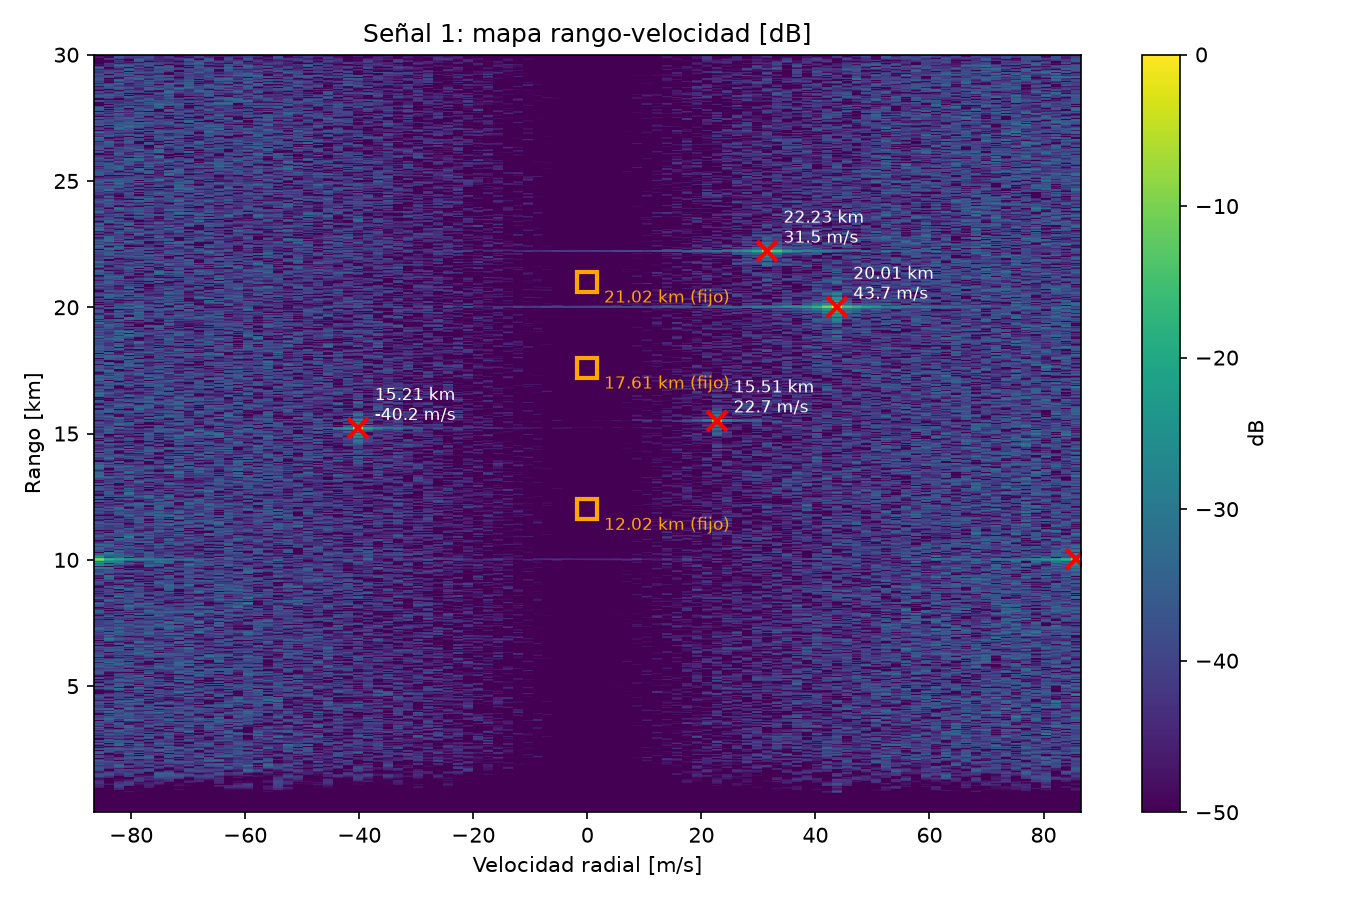
\includegraphics[height=0.82\textheight]{senal_1/08_mapa_rango_velocidad.png}
  \note{\textbf{Luca Baccino:} Este es el mapa rango-velocidad de la señal 1, en dB. Cada cruz roja es un blanco móvil en su distancia y su velocidad, y los cuadrados naranjas son los fijos, en velocidad cero. Se ve que el blanco de 15,51 km, que los canceladores no separaban, tiene otra velocidad que el de 15,21: uno se aleja a 22,7 metros por segundo y el otro se acerca a 40. El de 10 km está en el borde izquierdo, a menos 85,7, justo en el límite de la velocidad no ambigua.}
\end{frame}

\begin{frame}{Señal 1: blancos detectados}
  \centering
  \small
  \renewcommand{\arraystretch}{1.15}
  \begin{tabular}{crrrrl}
    \toprule
    \textbf{N.°} & \textbf{Rango [km]} & \textbf{$v_r$ [m/s]} & \textbf{$v_r$ [km/h]} & \textbf{SNR [dB]} & \textbf{Tipo} \\
    \midrule
    1 & 10,02 & $-85{,}7$ & $-308$ & 32,8 & Móvil (*) \\
    2 & 12,02 & 0 & 0 & -- & Fijo \\
    3 & 15,21 & $+40{,}2$ & $+145$ & 38,9 & Móvil \\
    4 & 15,51 & $-22{,}7$ & $-82$ & 37,9 & Móvil \\
    5 & 17,61 & 0 & 0 & -- & Fijo \\
    6 & 20,01 & $-43{,}7$ & $-157$ & 42,2 & Móvil \\
    7 & 21,02 & 0 & 0 & -- & Fijo \\
    8 & 22,23 & $-31{,}5$ & $-113$ & 39,2 & Móvil \\
    \bottomrule
  \end{tabular}
  \vspace{0.2cm}

  \raggedright\footnotesize
  \textbf{8 blancos: 5 móviles y 3 fijos.} $v_r > 0$: se acerca; $v_r < 0$: se aleja. \\
  (*) En el borde de $\pm 86{,}5$ m/s: podría estar replegada ($+87{,}4$ m/s).
  \note{\textbf{Luca Baccino:} El resultado de la señal 1 son ocho blancos: cinco móviles y tres fijos. La velocidad positiva es de acercamiento y la negativa de alejamiento. El blanco de 10 km tiene una velocidad en el borde del intervalo no ambiguo, así que podría ser en realidad uno que se acerca a 87 metros por segundo; para saberlo haría falta una segunda PRF. Descartamos además tres detecciones débiles en 1,5, 6,2 y 13,7 km que ningún cancelador confirmaba. Le paso a Joaquín con la señal 2.}
\end{frame}

% =====================================================
\section[Señal 2]{Señal 2}
\orador{Grupo Oeste}{Joaquín Monja}
\begin{frame}{Señal 2: CFAR del STI simple cancelador}
  \begin{columns}[c]
    \begin{column}{0.5\textwidth}
      \centering
      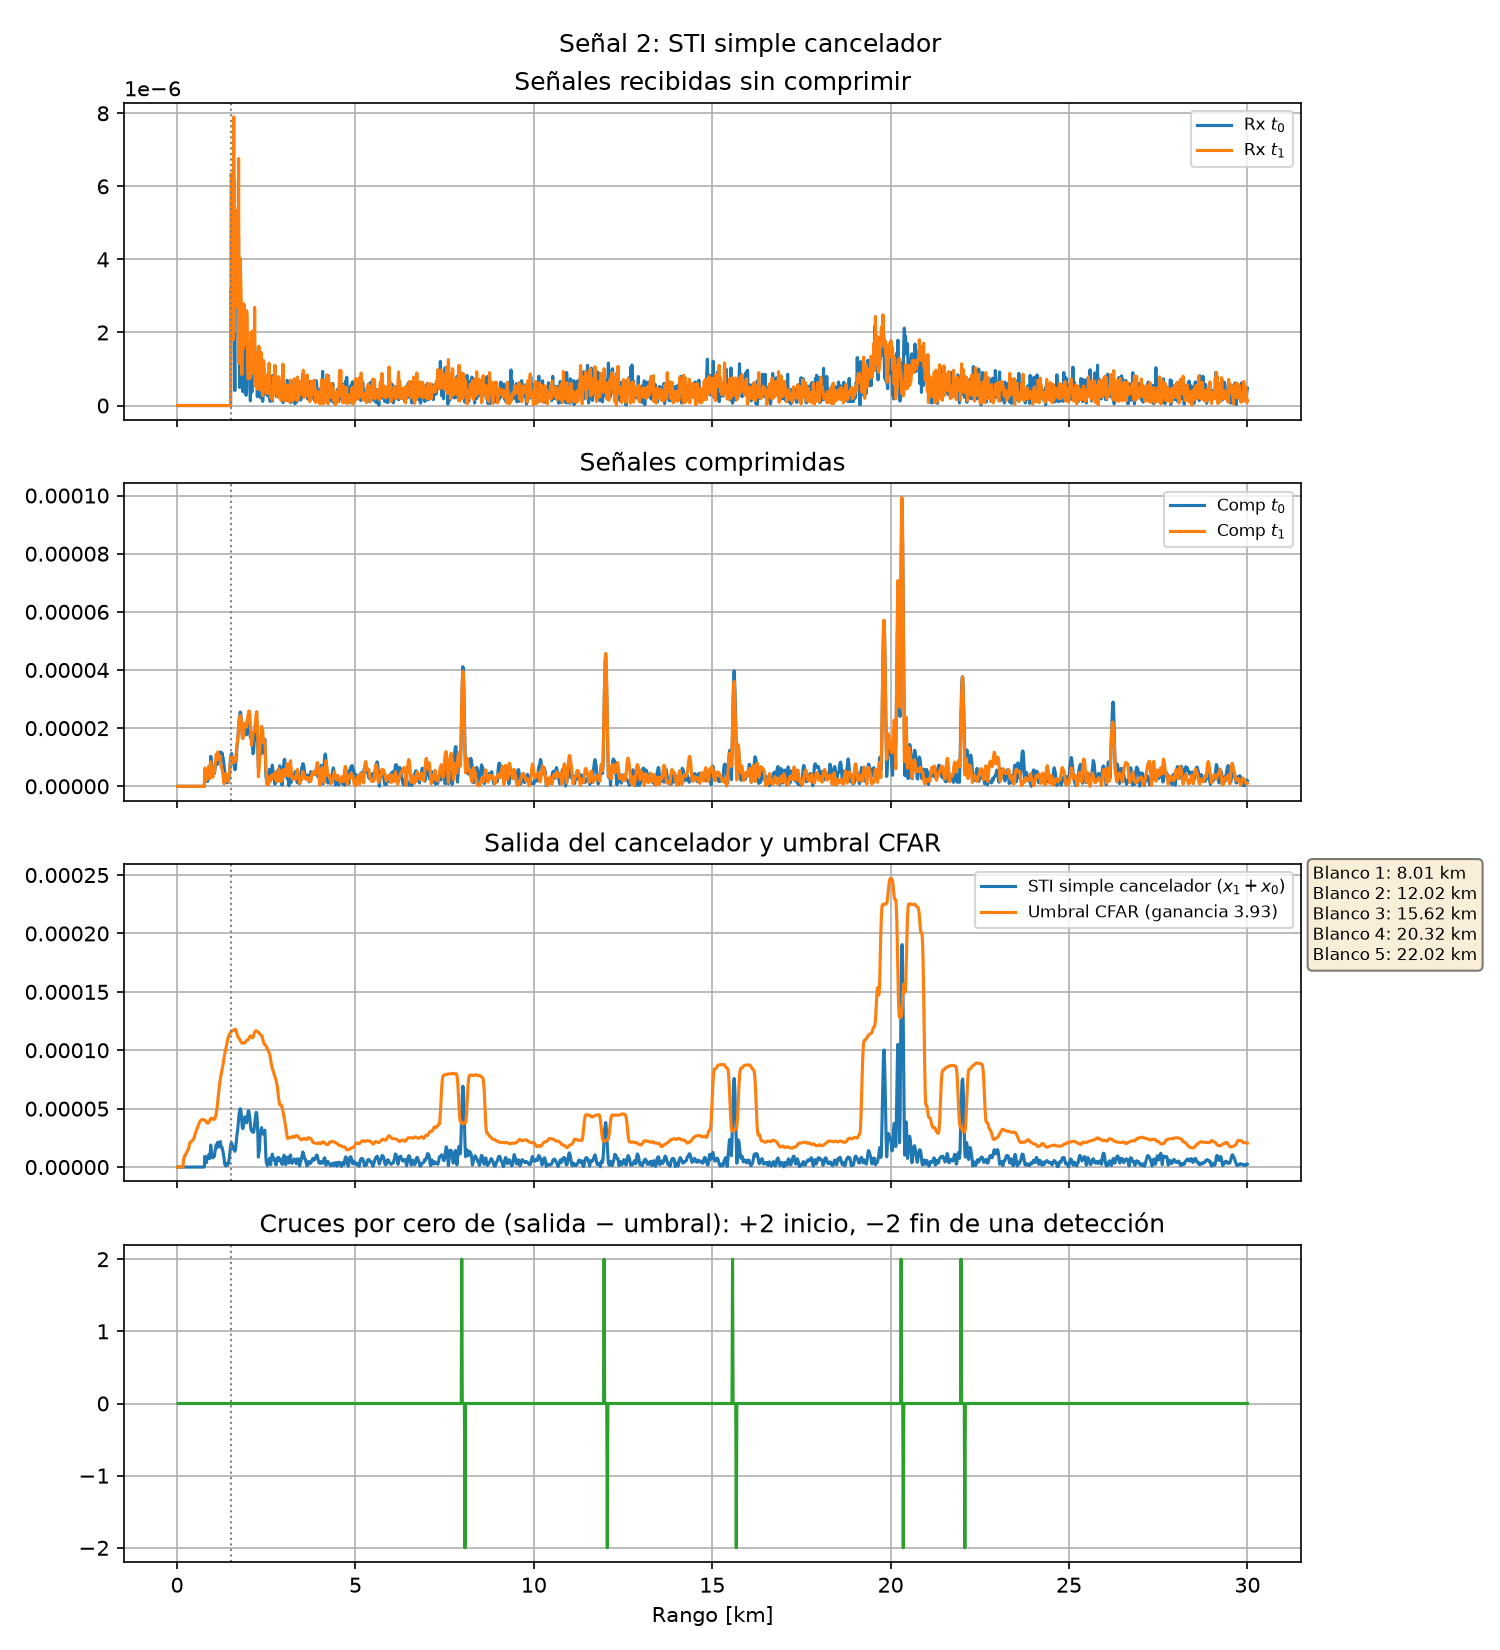
\includegraphics[height=0.86\textheight]{senal_2/05_cfar_sti_sc.png}
    \end{column}
    \begin{column}{0.5\textwidth}
      \small
      \textbf{Rangos detectados [km]:}
      \begin{itemize}
        \item MTI simple y doble: 8,01 -- 12,02 -- 20,22 -- 26,23
        \item STI simple: 8,01 -- 12,02 -- 15,62 -- 20,31 -- 22,02
      \end{itemize}
      \begin{itemize}
        \item El STI no ve el de 26,23 km: $f_D = +742$ Hz, en su nulo.
        \item 19,82 km tiene de las mayores SNR, pero \textbf{ningún cancelador lo detecta}: los ecos de 20,2--20,3 km le elevan el umbral.
        \item Con 200 celdas también se perdía el fijo de 22,02 km.
      \end{itemize}
    \end{column}
  \end{columns}
  \note{\textbf{Joaquín Monja:} En la señal 2 aplicamos exactamente el mismo procesamiento. Acá mostramos el STI, con su umbral. El MTI simple y el doble detectan cuatro móviles, en 8, 12, 20,2 y 26,2 km, y el STI detecta los tres fijos en 15,6, 20,3 y 22 km. Igual que en la señal 1, hay un blanco que el STI no ve porque cae en su nulo, el de 26 km. Y el caso más interesante es el de 19,8 km: es de los más fuertes, pero ningún cancelador lo detecta, porque los ecos de 20,2 y 20,3 km, a 400 metros, caen en su ventana de referencia y le suben el umbral. Con la ventana de 200 celdas era peor: también se perdía el fijo de 22 km.}
\end{frame}

\begin{frame}{Señal 2: mapa rango-velocidad}
  \centering
  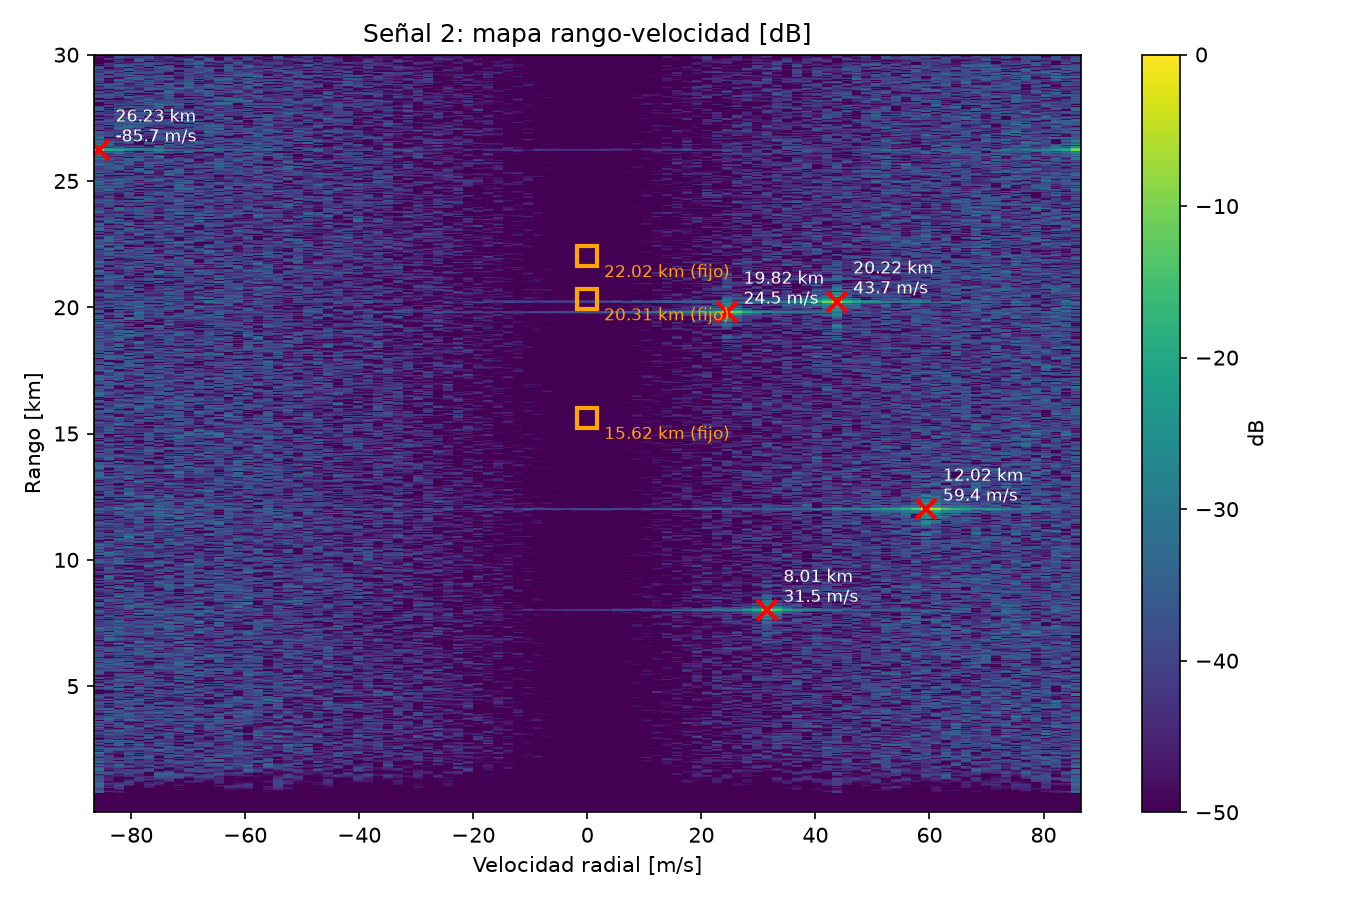
\includegraphics[height=0.82\textheight]{senal_2/08_mapa_rango_velocidad.png}
  \note{\textbf{Joaquín Monja:} En el mapa rango-velocidad de la señal 2 el blanco de 19,82 km aparece claramente, separado del de 20,22 porque tienen velocidades distintas: menos 24,5 y menos 43,7 metros por segundo. Es el mismo efecto que en la señal 1: el Doppler separa blancos que en rango están demasiado cerca para el CFAR. También se ve que en 20,2 y 20,3 km conviven un móvil y un fijo casi en la misma celda; los distinguimos porque el STI tiene su máximo en 20,31 y el MTI en 20,22.}
\end{frame}

\begin{frame}{Señal 2: blancos detectados}
  \centering
  \small
  \renewcommand{\arraystretch}{1.15}
  \begin{tabular}{crrrrl}
    \toprule
    \textbf{N.°} & \textbf{Rango [km]} & \textbf{$v_r$ [m/s]} & \textbf{$v_r$ [km/h]} & \textbf{SNR [dB]} & \textbf{Tipo} \\
    \midrule
    1 & 8,01 & $-31{,}5$ & $-113$ & 39,5 & Móvil \\
    2 & 12,02 & $-59{,}4$ & $-214$ & 40,6 & Móvil \\
    3 & 15,62 & 0 & 0 & -- & Fijo \\
    4 & 19,82 & $-24{,}5$ & $-88$ & 42,7 & Móvil \\
    5 & 20,22 & $-43{,}7$ & $-157$ & 42,1 & Móvil \\
    6 & 20,31 & 0 & 0 & -- & Fijo \\
    7 & 22,02 & 0 & 0 & -- & Fijo \\
    8 & 26,24 & $+85{,}7$ & $+308$ & 33,2 & Móvil (*) \\
    \bottomrule
  \end{tabular}
  \vspace{0.2cm}

  \raggedright\footnotesize
  \textbf{8 blancos: 5 móviles y 3 fijos.} $v_r > 0$: se acerca; $v_r < 0$: se aleja. \\
  (*) En el borde de $\pm 86{,}5$ m/s: podría estar replegada ($-87{,}4$ m/s).
  \note{\textbf{Joaquín Monja:} La señal 2 también tiene ocho blancos, cinco móviles y tres fijos. El de 26,24 km está en el borde del intervalo no ambiguo, igual que el de 10 km de la señal 1 pero con el signo contrario, así que también podría estar replegado.}
\end{frame}

% =====================================================
\section[Conclusiones]{Conclusiones}
\orador{Grupo Oeste}{Joaquín Monja}
\begin{frame}{Comparación de las dos señales}
  \centering
  \small
  \renewcommand{\arraystretch}{1.2}
  \begin{tabular}{p{4.2cm}p{3.6cm}p{3.6cm}}
    \toprule
    & \textbf{Señal 1} & \textbf{Señal 2} \\
    \midrule
    Blancos & 5 móviles, 3 fijos & 5 móviles, 3 fijos \\
    Fijos [km] & 12,02 -- 17,61 -- 21,02 & 15,62 -- 20,31 -- 22,02 \\
    Velocidad en el nulo del STI & 10,02 km ($-85{,}7$ m/s) & 26,24 km ($+85{,}7$ m/s) \\
    Enmascarado en CFAR & 15,51 km (a 300 m) & 19,82 km (a 400 m) \\
    Recuperado por & Doppler & Doppler \\
    \bottomrule
  \end{tabular}
  \vspace{0.3cm}

  \raggedright\small
  En las dos aparecen las mismas falsas alarmas (1,5, 6,2 y 13,7 km): las simulaciones comparten la realización del ruido.
  \note{\textbf{Joaquín Monja:} Si comparamos las dos señales, tienen la misma estructura: cinco móviles y tres fijos. En las dos hay un blanco con velocidad cerca del borde, que el STI no ve, y en las dos hay un blanco enmascarado por un vecino a pocos cientos de metros, que solo se recupera con el Doppler. Un detalle curioso: las tres falsas alarmas aparecen en las mismas distancias en las dos señales y en la de ejemplo, lo que indica que las simulaciones usan el mismo ruido.}
\end{frame}

\begin{frame}{Conclusiones}
  \small
  \begin{itemize}
    \item \textbf{Compresión:} imprescindible. Sin ella los ecos quedan bajo el ruido y ocupan 1,5 km; comprimidos ganan 13 dB y se resuelven con 75 m.
    \item \textbf{Canceladores:} el MTI elimina clutter y ecos fijos; el STI los refuerza; el MTI doble ensancha el nulo. Sus nulos generan velocidades ciegas.
    \item \textbf{CA-CFAR:} mantiene la tasa de falsas alarmas, pero un blanco fuerte enmascara a los vecinos de su ventana. 64 celdas de referencia y 8 de guarda funcionaron mejor que 200.
    \item \textbf{Doppler:} aporta la velocidad, unos 20 dB de integración coherente y separa blancos cercanos en rango. Fue la detección más robusta.
    \item \textbf{PRF de 1500 Hz:} limita la velocidad no ambigua a $\pm 86{,}5$ m/s. Para resolver los blancos del borde haría falta una segunda PRF.
  \end{itemize}
  \note{\textbf{Joaquín Monja:} Para cerrar. La compresión con el filtro apareado fue imprescindible: sin ella no se ve ningún blanco. Los canceladores se complementan: el MTI deja los móviles y el STI los fijos, aunque cada uno tiene velocidades en las que no ve nada. El CFAR adapta el umbral al ruido, pero un blanco fuerte tapa a sus vecinos, y por eso elegir el tamaño de la ventana es un compromiso. El procesamiento Doppler fue lo más robusto: da la velocidad, suma 20 dB y separa los blancos que el CFAR no podía. Y la PRF limita las velocidades que podemos medir sin ambigüedad: para los blancos del borde haría falta una segunda PRF.}
\end{frame}

\begin{frame}[plain]
  \begin{tikzpicture}[remember picture, overlay]
    \fill[unc verde] (current page.north west) rectangle (current page.south east);
    \node[text=white, font=\Huge\bfseries] at (current page.center) {¡Gracias!};
    \node[text=white, font=\large] at ([yshift=-1.2cm]current page.center) {¿Preguntas?};
  \end{tikzpicture}
  \note{\textbf{Joaquín Monja:} Muchas gracias. Si tienen preguntas, las respondemos entre todos.}
\end{frame}
